\chapter{Linked List}


\section{Operations}
\subsection{Fundamentals}
Get the $pre$ reference:
\begin{python}
dummy = Node(0)
dummy.next = head
pre = dummy
cur = pre.next
\end{python}

\subsection{Basic Operations}
\begin{enumerate}
\item Get the length
\item Get the $i$-th object
\item Delete a node 
\item Reverse
\begin{figure}[H]
\centering
\subfloat{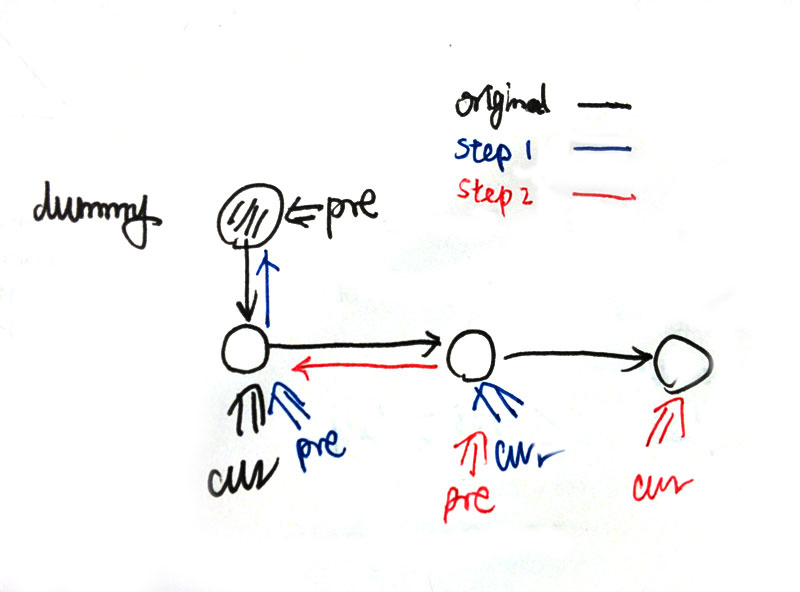
\includegraphics[scale=1.0]{ll_reverse}}
\caption{Reverse the linked list}
\label{fig:LABEL}
\end{figure}
\begin{python}
def reverseList(self, head):
    dummy = ListNode(0)
    dummy.next = head

    pre = dummy
    cur = pre.next
    while pre and cur:
        pre, cur.next, cur = cur, pre, cur.next
        # incorrect evaluation order
        # pre, cur, cur.next = cur, cur.next, pre 

    dummy.next.next = None  # original head
    return pre  # new head
\end{python}
Notice: the evaluation order for the swapping the nodes and links. 
\end{enumerate}

\subsection{Combined Operations}
In $O(n)$ without extra space:
\begin{enumerate}
\item Determine whether two lists intersects
\item Determine whether the list is palindrome 
\item Determine whether the list is acyclic
\end{enumerate}
